\documentclass{article}
\usepackage[a4paper, margin=2cm]{geometry}

\usepackage[utf8]{inputenc} % allow utf-8 input
\usepackage[T1]{fontenc}    % use 8-bit T1 fonts
\usepackage{hyperref}       % hyperlinks
\hypersetup{
    colorlinks,
    linkcolor={red!50!black},
    citecolor={blue!50!black},
    urlcolor={blue!80!blue}
}
\usepackage{xcolor}
\usepackage{nicefrac}       % compact symbols for 1/2, etc.
\usepackage{bm, bbm}
\usepackage{physics, tensor}

\usepackage{amsmath}
\usepackage{amssymb}
\usepackage{mathtools}
\usepackage{amstext}
\usepackage{amsthm}
\usepackage{linop}
\usepackage{tikz}
\usetikzlibrary{snakes}
\usetikzlibrary{arrows.meta,decorations.markings}



\usepackage{fancyhdr}
\pagestyle{fancy}
\rhead{Alexandre Adam\\ 20090755}
\lhead{William Witczak-Krempa \\ PHY 6812: Théorie des champs 1}
\chead{Devoir 2}
\rfoot{1\textsuperscript{er} novembre 2022}
\cfoot{\thepage}

\numberwithin{equation}{section}
\renewcommand\thesubsection{\alph{subsection})}
\renewcommand\thesubsubsection{\Roman{subsubsection}}
\DeclareRobustCommand{\bbone}{\text{\usefont{U}{bbold}{m}{n}1}}

\begin{document}
\section{Causalité}
\subsection{}
\textbf{Dans la preuve que la QFT du champ scalaire respecte la causalité, nous avons utilisé la propriété que $x - y$ peut être envoyé à $- (x -  y)$ par une transformation de Lorentz 
connectée de manière continue à l’identité, en autant que la séparation est du genre espace.
On cherche la transformation de Lorentz explicite pour cette transformation, et on cherche à 
démontrer que la construction échoue si $(x - y)^{2} > 0$ (une séparation de genre temps), avec $d=3$ dimensions spatiales.}\\

On suppose sans perte de généralité que $(x - y) = (t, x, 0, 0)$. On cherche à amener ce vecteur à $-(x - y) =(-t, -x, 0, 0)$. 
Pour ce faire, on considère en premier lieu un boost en terme de la rapidité $\zeta \in \mathbb{R}$
\begin{align}
        t' &= t \cosh \zeta - x \sinh \zeta \\
        x' &= -t \sinh \zeta + x\cosh \zeta
\end{align}
%On pose $t' = -t$, de sortes que
Pour faire passer $t \rightarrow -t$, on doit d'abord passer par $t' = 0$. Vérifions que cela est possible
\begin{align*}
       t' = 0 \implies \tanh \zeta = \frac{t}{x} 
\end{align*}
\textbf{Cette équation n'a pas de solution si $x > t$, soit le cas où $(x - y)^2 > 0$. 
Autrement dit, la séparation $(x - y)$ doit être de type spatiale, $(x - y)^2 < 0$ pour que 
la construction existe}. Supposons maintenant que la séparation est de type spatiale. La construction se fait en 3 étapes
\paragraph{Boost dans la direction $y$:} On pose la rapidité de la transformation $\zeta = \tanh^{-1}\frac{t}{y}$, de sortes que
\begin{align*}
        t' &= 0 \\
        x' &= x \\
        y' &= t \cosh \zeta - y \sinh \zeta
\end{align*}
\paragraph{Rotation par $\pi$ selon l'axe $z$:} 
\begin{align*}
        t'' &= 0 \\
        x'' &= -x' = -x \\
        y'' &= -y'
\end{align*}
\paragraph{Inverse du premier boost:}
\begin{align*}
        x''' &= x'' = -x \\
        t''' &= t'' \cosh \zeta + y'' \sinh \zeta \\
             &= -y' \sinh \zeta \\
             &= t\sinh^2 \zeta - y\cosh \zeta \sinh \zeta \\
             &= \cosh^2 \zeta (t\tanh^2 \zeta - y \tanh \zeta) \\
             &= t\cosh^2 \zeta (\tanh^2 \zeta - 1) \hspace{1cm} \big\{ \tanh \zeta = \frac{t}{y} \big\}\\
             &= -t \hspace{3.8cm} \big\{\cosh^2\zeta = \frac{1}{1 - \tanh^2\zeta} \big\}\\
        y''' &= t'' \sinh \zeta + y'' \cosh \zeta \\
             &= -y' \cosh \zeta \\
             &= t \sinh \zeta\cosh \zeta - y\cosh^2 \zeta  \\
             &= \cosh^2\zeta \left(t \frac{1}{\tanh \zeta} - y \right)  \\
             &= \cosh^2\zeta \left( y  - y \right)  \\
             &= 0
\end{align*}
Le résultat de cette transformation est $\Lambda(x - y) = -(x - y) = (-t, -x, 0, 0)$.


\subsection{}
\textbf{Pour $(x - y)^2 > 0$, on cherche une transformation de Lorentz qui envoie $(x - y) \rightarrow  -(x - y)$.
Est-elle connectée de manière continue à l’identité? Pourquoi ne peut-on pas l’utiliser pour
montrer que $[ \hat{\phi}(x), \hat{\phi}(y)] = 0$ pour une séparation du genre temps?} \\
La transformation de Lorentz qui transforme $(x - y) -> -(x - y)$ est la matrice $PT$:
\begin{equation}
        PT = \begin{pmatrix}
                -1 & 0   \\
                0 & -\bbone
        \end{pmatrix}
\end{equation} 
Soit le résultat de l'application combinée de la parité spatiale
\begin{equation}
        P = \begin{pmatrix}
                1 & 0 \\
                0 & -\bbone
        \end{pmatrix}
\end{equation} 
et de la parité temporelle
\begin{equation}
        T = \begin{pmatrix}
                -1 & 0 \\
                0 & \bbone
        \end{pmatrix}
\end{equation} 
De façon intéressante, le déterminant $\det(PT) = 1$, ce qui suggère que la matrice pourrait être connectée à l'identité. Or, puisqu'il est impossible 
de construire $PT$ à partir d'une combinaison de boosts ou de matrice rotation, autrement dit les matrices du groupe $SO^{+}(3, 1)$, alors 
la matrice $PT$ ne peut pas être connectée à l'identité. \textbf{Puisque seuls les transformations discrètes du groupe $O(3, 1)$ ($O(3, 1) / SO^{+}(3, 1)$) sont connectées 
à la matricé $PT$, alors la matrice $PT$ n'est pas connectée de façon continue à l'identité pour une séparation de genre temps.} \\

Finalement, on illustre pourquoi cette transformation ne peut pas être utilisée pour démontrer que ${[\hat{\phi}(x),\hat{\phi}(y)] = 0}$ lorsque $(x - y)^{2} > 0$.



\section{}
\subsection{}
\textbf{Montrez que les opérateurs $\hat{a}_\mathbf{p}$ commutent entre eux.} \\

Pour ce faire, on suppose les relations de commutations canoniques pour les champs $\phi(\mathbf{x})$ et $\pi(\mathbf{x})$:
\begin{equation}
        [\phi(\mathbf{x}), \pi(\mathbf{y})] = i\delta^{(n)}(\mathbf{x} - \mathbf{y})
\end{equation} 
et
\begin{equation}
        [\phi(\mathbf{x}), \phi(\mathbf{y})] = [\pi(\mathbf{x}), \pi(\mathbf{y})] = 0
\end{equation} 
On pose
\begin{align}
        \phi(\mathbf{p}) &= \int \frac{d^{n}\mathbf{x}}{(2\pi)^{n}}\, e^{-i \mathbf{p}\cdot \mathbf{x}} \phi(\mathbf{x}) \\
        \pi(\mathbf{p}) &= \int \frac{d^{n}\mathbf{x}}{(2\pi)^{n}} e^{-i \mathbf{p} \cdot \mathbf{x}} \pi(\mathbf{x}) \\
        a_{\mathbf{p}} &= \frac{1}{\sqrt{2 \omega_{\mathbf{p}}}}(\omega_{\mathbf{p}}\phi(\mathbf{p}) + i \pi(\mathbf{p}))
\end{align} 
De sortes que
\begin{align*}
        [a_{\mathbf{p}}, a_{\mathbf{q}}] &= 
        \frac{1}{2\sqrt{\omega_{\mathbf{p}} \omega_{\mathbf{q}}}}\int_{\mathbf{x}} \int_{\mathbf{y}}
        e^{-i \mathbf{x} \cdot \mathbf{p}}e^{-i \mathbf{y} \cdot \mathbf{q}}
[\omega_{\mathbf{p}} \phi(\mathbf{x}) + i \pi(\mathbf{x}),\, \omega_{\mathbf{q}} \phi(\mathbf{y}) + i \pi(\mathbf{y})] \\
        &= \frac{1}{2\sqrt{\omega_{\mathbf{p}} \omega_{\mathbf{q}}}}\int_{\mathbf{x}} \int_{\mathbf{y}}
        e^{-i \mathbf{x} \cdot \mathbf{p}}e^{-i \mathbf{y} \cdot \mathbf{q}}
        \big(
              \omega_{\mathbf{q}} \delta^{(n)}(\mathbf{x} - \mathbf{y}) -\omega_{\mathbf{p}} \delta^{(n)}(\mathbf{x} - \mathbf{y})
\big) \\
        &= \frac{1}{2\sqrt{\omega_{\mathbf{p}} \omega_{\mathbf{q}}}}\int_{\mathbf{x}}
        e^{-i\mathbf{x} \cdot( \mathbf{p} + \mathbf{q})} 
        \big(
              \omega_{\mathbf{q}} -\omega_{\mathbf{p}}
\big) \\
        &= \frac{1}{2\sqrt{\omega_{\mathbf{p}} \omega_{\mathbf{q}}}}
        (2\pi)^{n}\delta^{(n)}(\mathbf{p} + \mathbf{q})
        \big(
              \omega_{\mathbf{q}} -\omega_{\mathbf{p}}
\big) \\
&=  0
\end{align*}
Puisque $\omega_{\mathbf{p}} = \omega_{-\mathbf{p}}$.

\subsection{}
\textbf{Soit deux observables classiques $A$ et $B$. Considérons l’observable $\mathcal{O} = AB$. 
En quantifiant la théorie, il y a une ambiguité potentielle pour $\hat{\mathcal{O}}$ du fait que $\hat{A}$ et $\hat{B}$ ne commutent
pas nécessairement. Cette ambiguité pose-t-elle problème pour l’opérateur d’impulsion totale $\hat{P}$ ?} \\

%L'opérateur d'impulsion totale
On s'intéresse à l'ambigüité qui provient de l'ordre des opérateur. En particulier, considérons l'impulsion, 
soit la charge de Noether globale qui correspond à une symétrie de translation, pour une théorie classique
\begin{equation}
        P_i = \int d^{n}\mathbf{x}\, \pi(\mathbf{x}, t) \partial_i \phi(\mathbf{x}, t)
\end{equation} 
Clairement, il y a une ambigüité lorsqu'on fait la quantification de cette opérateur, puisque les opérateurs 
$\op{\pi}{}{}$ et $\partial_i\op{\phi}{}{}$ ne commutent pas nécessairement pour une théorie donnée. En général, 
l'ordre normal est adopté, de sortes que
\begin{equation}
        :P_i: = \int d^{n}\mathbf{x} \, \op{\pi}{}{}(\mathbf{x}, t) \partial_i \op{\phi}{}{}(\mathbf{x}, t)
\end{equation} 
Toutefois, ce n'est pas la solution unique à la quantification, puisque $\pi(\mathbf{x}, t)$ et $\partial_i \phi(\mathbf{x}, t)$ commutent dans 
la théorie classique.


\subsection{}
\textbf{En travaillant dans le point de vue de Schrödinger avec la théorie de Klein-Gordon,
on veut déterminer l’évolution temporelle de l’état $b_0 | 0 \rangle + b_1 | p \rangle + b_2 | p, q, k \rangle $, où $b_0,b_1,b_2 \in \mathbb{C}$ et $p, q, k$ des quadri-vecteurs.}\\ 
%L'Hamiltonien de la théorie de Klein-Gordon dans son espace propre est
%\begin{align*}
        %H = \int \frac{d^{3}\mathbf{p}}{(2\pi)^{3}}\, E_{\mathbf{p}}a^{\dagger}_{\mathbf{p}}a_{\mathbf{p}}
%\end{align*}
%Ce qu'on peut réécrire en terme d'une intégrale dans l'espace-temps comme
%\begin{equation}
        %H = \int \frac{d^{4} p}{(2\pi)^{4}}\, E_{\mathbf{p}}a^{^{\dagger}}_{\mathbf{p}}a_{\mathbf{p}} (2\pi) \delta(p^{0} - E_{\mathbf{p}})
%\end{equation} 
%Selon l'équation de Schrödinger
On applique l'équation de Schrödinger pour déterminer l'évolution temporelle de l'état
\begin{align*}
        H(b_0 | 0 \rangle + b_1 | p \rangle + b_2 | p, q, k \rangle  ) &= b_1 
\end{align*}

\subsection{}
\textbf{Est-ce possible de construire un état normalisable dans le sous-espace à 1 particule? 
%Si non, expliquez, si oui, construisez un état normalisé.
}
\section{Invariance d'échelle quantique}
Soit la QFT du champ scalaire Klein-Gordon sans masse
en 3 dimensions spatiales. Considérons une transformation continue :
\begin{equation}
        \begin{split}
                x &\rightarrow bx, \\
                \hat{\phi}(x) &\rightarrow b^{-\Delta} \hat{\phi}(x)
        \end{split}
\end{equation} 
où $b \in \mathbb{R}_{>0}$ et $\Delta \in \mathbb{R}$.

\subsection{}
\subsubsection{Amplitude pour l'opérateur de champ}
On veut évaluer l'amplitude 
\begin{equation}
        D(x - y) = \langle 0 | \hat{\phi}(x) \hat{\phi}(y) | 0 \rangle  
\end{equation} 
Pour ce qui suit, je vais omettre les chapeaux pour alléger la notation.
On utilise les relations canoniques de commutation pour les 
opérateurs d'échelles, $[a_{\mathbf{p}}, a^{\dagger}_{\mathbf{q}}] = (2\pi)^{3}\delta^{(3)}(\mathbf{p} - \mathbf{q})$, 
ainsi que l'expansion de Fourier
\begin{align}
        \phi(x) = \int \frac{d^{3}\mathbf{p}}{(2\pi)^{3}}\, e^{-i p \cdot x}\frac{1}{\sqrt{2E_{\mathbf{p}}}}(a_{\mathbf{p}} + a^{\dagger}_{-\mathbf{p}})\bigg|_{p^{0} = E_{\mathbf{p}}}
\end{align}
pour les opérateurs de positions. On calcule l'amplitude $D(x - y)$ évaluée sur la coquille d'énergie $p^{0} = E_{\mathbf{p}}$, 
\begin{align*}
        D(x - y) &= \int_{\mathbf{p}} \int_{\mathbf{q}} \frac{1}{2\sqrt{E_{\mathbf{p}}E_{\mathbf{q}}}}
        \langle 0 |  (a_{\mathbf{p}}e^{-i p\cdot x} + a^{\dagger}_{\mathbf{p}}e^{i p\cdot x})(a_{\mathbf{q}}e^{-i q \cdot y} + a^{\dagger}_{\mathbf{q}}e^{i q\cdot y})
        | 0 \rangle 
        \bigg|_{\substack{p^{0} = E_{\mathbf{p}} \\ q^{0} = E_{\mathbf{q}}}} \\
        &= \int_{\mathbf{p}} \int_{\mathbf{q}} \frac{1}{2\sqrt{E_{\mathbf{p}}E_{\mathbf{q}}}}
        e^{-i p \cdot x + i q\cdot y}
        \langle 0 | a_{\mathbf{p}}a^{\dagger}_{\mathbf{q}} | 0 \rangle 
        \bigg|_{\substack{p^{0} = E_{\mathbf{p}} \\ q^{0} = E_{\mathbf{q}}}} \\
        &= \int_{\mathbf{p}}  \frac{1}{2E_{\mathbf{p}}}
        e^{-i p \cdot (x - y)}\bigg|_{p^{0} = E_{\mathbf{p}}} 
\end{align*}
où on a simplifier l'expression en appliquant les opérateurs d'annihilation sur l'état fondamental $a_{\mathbf{p}} | 0 \rangle = \langle 0 |a^{\dagger}_{\mathbf{p}} = 0  $ 
et en appliquant le commutateur canonique. Dans le système de coordonnées sphériques, on introduit ${(x - y) = (t, \mathbf{r})}$, le quadri-vecteur 
de séparation, de sortes que
\begin{align*}
        D(x - y) &= \frac{1}{2(2\pi)^{3}} \int_{0}^{\infty }dp\, p^2 \int_0^{\pi} d\theta\, \sin\theta \int_0^{2\pi}d\phi\,  \frac{1}{E_p}e^{i p r \cos\theta - E_{p}t}
        \\
                 &=  \frac{1}{2(2\pi)^{2}} \int_{0}^{\infty }dp\, p^2 \int_{-1}^{1}d(\cos \theta)\,  \frac{1}{E_p}e^{i p r\cos\theta  - E_{p}t} \\
                 &=   \frac{1}{8\pi^2} \int_{0}^{\infty }dp\, p^2   \frac{1}{E_p} \frac{1}{ipr}(e^{ipr} - e^{-ipr})e^{-iE_pt} \\
                 &=   \frac{1}{8\pi^2ir}\frac{1}{2}\int_{-\infty }^{\infty }dp\, p   \frac{1}{E_p}(e^{ipr} - e^{-ipr}) e^{-iE_pt} \\
                 &=   \frac{1}{8\pi^2ir}  \int_{-\infty }^{\infty }dp\, p   \frac{1}{\sqrt{p^2 + m^2}}e^{ipr} e^{-i\sqrt{p^2 + m^2}t} 
\end{align*}
où on a exploiter la parité paire de $p(e^{ipr} - e^{-ipr})$ et $E_{p}$ pour étendre la région d'intégration $\int_{0}^{\infty} \rightarrow \frac{1}{2}\int_{-\infty }^{\infty }$, 
et finalement on a exploiter la symétrie des bornes d'intégrations pour simplifier l'intégrale.
Pour poursuivre, on doit choisir un contour d'intégration, ce qui nécessite aussi de déterminer la variété de Minkowsky 
sur laquelle on intègre. 

\begin{figure}
\centering
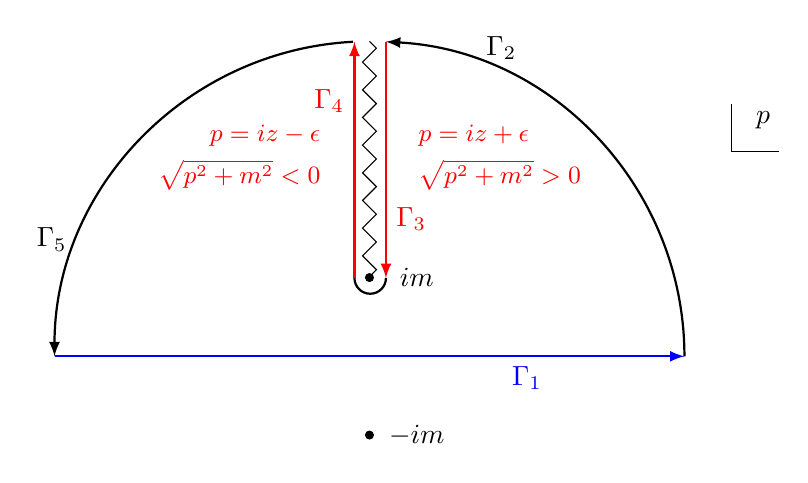
\begin{tikzpicture}
        \node at (5, 3) {$p$};
        \draw (4.6, 2.6) -- (5.2, 2.6);
        \draw (4.6, 2.6) -- (4.6, 3.2);
        \draw[-latex, thick, color=blue] (-4, 0) -- (4, 0) node[near end, below, color=blue] {$\Gamma_1$};
        \node[circle, draw=black, inner sep=1pt, fill=black] (-im) at (0, -1) {};
        \node at (0.6, -1) {$-im$};
        \node[circle, draw=black, inner sep=1pt, fill=black] (-im) at (0, 1) {};
        \node at (0.6, 1) {$im$};
        \draw[-latex, draw=black, thick] (4, 0) arc (0: 87: 4) node[near end, above] {$\Gamma_2$};
        \draw[snake=zigzag] (0, 4) -- (0, 1); 
        \draw[-latex, draw=red, thick] (87:4) -- +(0, -3) coordinate (temp1) node[near end, right, color=red] {$\Gamma_3$};
        \draw[draw=red, thick, color=black] (temp1) arc (0:-180:.2) coordinate (temp2);
        \draw[-latex, draw=red, thick, color=red] (temp2) -- ++(0, 3) coordinate (temp3) node[near end, left, color=red] {$\Gamma_4$};
        \draw[latex-, draw=black, thick] (-4, 0) arc (180:93:4) node[near start, left] {$\Gamma_5$};
        \node[anchor=west, color=red] at (.5, 2.8) {\small$p = iz + \epsilon$};
        \node[anchor=west, color=red] at (.5, 2.3) {\small$\sqrt{p^2 + m^2} > 0$};
        \node[anchor=east, color=red] at (-.5, 2.8) {\small$p = iz - \epsilon$};
        \node[anchor=east, color=red] at (-.5, 2.3) {\small$\sqrt{p^2 + m^2} < 0$};
        %\node[anchor=west] at (4.1, 1) {$e^{i(pr - \sqrt{p^2 + m^2}t)} \rightarrow 0$};
        %\node[anchor=west] at (4.1, .3) {Lorsque $r > t \geq 0$ et $p \rightarrow i\infty $};
        
\end{tikzpicture}
\caption{Contour d'intégration pour une séparation de type espace.}
\label{fig:contour1}
\end{figure}

\paragraph{Séparation de type espace:} On considère le cas où $r > t \geq 0$. 
Dans ce cas, on choisit un contour d'intégration antihoraire dans le demi-plan supérieur complexe pour évaluer l'intégrale. 
Ce contour est choisit tels que $e^{i(pr - \sqrt{p^2 + m^2}t)} \rightarrow e^{ipr}  \rightarrow 0$ lorsque $p \rightarrow  i\infty $, de sortes que 
les contours $\Gamma_2$ et $\Gamma_5$ ne contribuent pas à l'intégrale.
Les seules contributions non nulles à l'intégrale de Cauchy proviennent 
des segments $\Gamma_1$, $\Gamma_3$ et $\Gamma_4$ (voir figure \ref{fig:contour1}). Sur le contour $\Gamma_3$, la racine $\sqrt{p^2 + m^2}$ devient 
positive imaginaire, alors que sur le contour $\Gamma_4$ la racine devient négative imaginaire. Puisqu'il n'y aucune 
singularité à l'intérieur du contour, l'intégrande est holomorphique et $\oint_\Gamma = 0$, de sortes que
\begin{align*}
        D(x - y) &= \int_{\Gamma_1}= -\bigg(\int_{\Gamma_3 } +\int_{\Gamma_4}\bigg)\\
        &= - \frac{1}{8\pi^2ir}
        \begin{aligned}[t]
                \bigg(&\int_{\infty }^{m} d(iz)\, (iz)   \frac{1}{i\sqrt{z^2 - m^2}} e^{-zr} e^{\sqrt{z^2 - m^2}t}  \\
                      & + \int_{m}^{\infty}d(iz)\, (iz) \frac{1}{-i\sqrt{z^2 - m^2}}e^{-zr} e^{-\sqrt{z^2 - m^2}t} \bigg)
        \end{aligned}\\
        %&= - \frac{1}{8\pi^2r}
        %\begin{aligned}[t]
                %\bigg(&\int_{\infty }^{m} dz\, z   \frac{1}{\sqrt{z^2 - m^2}} e^{-zr} e^{\sqrt{z^2 - m^2}t}  \\
                      %& - \int_{m}^{\infty}dz\, z\frac{1}{\sqrt{z^2 - m^2}}e^{-zr} e^{-\sqrt{z^2 - m^2}t} \bigg)
        %\end{aligned}\\
        &= \frac{1}{8\pi^2r}
                \int_{m }^{\infty } dz\, z   \frac{1}{\sqrt{z^2 - m^2}} e^{-zr}( e^{\sqrt{z^2 - m^2}t} 
                       +e^{-\sqrt{z^2 - m^2}t})\\
        &= \frac{1}{4\pi^2r}
        \int_{m }^{\infty } dz\, z   \frac{ e^{-zr}}{\sqrt{z^2 - m^2}}\cosh(\sqrt{z^2 - m^2}t)
\end{align*}
Pour simplifier l'intégrale, on utilise une transformation de Lorentz tels que $\Lambda(x - y) = (0, \mathbf{r})$. Ainsi,
\begin{align}
        \nonumber
D(\Lambda(x - y)) 
        &= \frac{1}{4\pi^2r}
        \int_{m }^{\infty } dz\, z   \frac{ e^{-zr}}{\sqrt{z^2 - m^2}}
\end{align}
Pour résoudre cette intégrale, on doit finalement la faire correspondre avec la représentation intégrale de la fonction de Bessel modifiée de deuxième 
type
\begin{equation}\label{eq:bessel2}
        K_{\nu}(z) = \frac{\sqrt{\pi} z^{\nu}}{2^{\nu}\Gamma(\nu + \frac{1}{2})} \int_{1}^{\infty } e^{-zt} (t^{2} - 1)^{\nu - \frac{1}{2}}dt
\end{equation} 
où $\Re(z) > 0$. Pour ce faire, on applique le changement de variable $t = z / m$, de sortes que
\begin{align*}
D(\Lambda(x - y))  &= \frac{m}{4\pi^2r} \int_{1}^{\infty } dt\, t \frac{ e^{-mtr}}{\sqrt{t^2 - 1}} \\
         &= -\frac{1}{4\pi^2r} \frac{\partial}{\partial r}\int_{1}^{\infty } dt\,\frac{ e^{-mtr}}{\sqrt{t^2 - 1}} \\
        &= -\frac{1}{4\pi^2r} \frac{\partial}{\partial r} \left(  \frac{\Gamma(\frac{1}{2}) }{\sqrt{\pi}} K_{0}(mr) \right)
\end{align*}
En utilisant le fait que $\Gamma(\frac{1}{2}) = \sqrt{\pi}$, on trouve
\begin{align*}
        D(\Lambda(x - y)) &= -\frac{1}{4\pi^2r} \frac{\partial}{\partial r} K_{0}(mr)
\end{align*}
On utilise maintenant une identité pour $K_\nu(z)$ qui relie les dérivées de $K_{\nu}$ avec d'autres 
fonctions de Bessel modifiées
\begin{align}\label{eq:bessel id1}
       \frac{\partial K_\nu(z)}{\partial z} = -\frac{1}{2}(K_{\nu-1}(z) + K_{\nu+1}(z)) 
\end{align}
Cette identité peut être démontrées aisément à partir de la représentation intégrale suivante
\begin{equation}
        K_{\nu}(z) = \int_{0}^{\infty } e^{-z \cosh(t)} \cosh(\nu t) dt
\end{equation} 
et du fait que $\cosh(t)\cosh(\nu t) = \frac{1}{2}(\cosh((\nu - 1) t) + \cosh((\nu + 1)t))$. On utilise aussi le fait que 
$K_{-\nu} = K_{\nu}$, de sortes que
\begin{align}
        \label{eq:spacelike}
        \implies \Aboxed{D(\Lambda(x - y)) &= \frac{m}{4\pi^2r}  K_1(mr) }
\end{align}
Ainsi, pour une séparation générale $(x - y) = (t, \mathbf{r})$ de type espace, 
on peut toujours évaluer $D(x - y)$ en trouvant la transformation de Lorentz tel que $\Lambda(x - y) = (0, \mathbf{r})$ et 
en utilisant l'équation \eqref{eq:spacelike}. \textbf{L'amplitude de propagation $D(x - y)$ est manifestement un invariant de Lorentz}. Ceci suit du fait 
que $p \cdot x$ et $\int \frac{d^{3} \mathbf{p}}{(2\pi)^{3}} \frac{1}{2E_{\mathbf{p}}}$ sont des invariants de Lorentz. \textbf{La représentation finale 
n'est pas manifestement invariante, puisqu'elle requiert de calculer $r$ dans le référentiel où $t = 0$}. Toutefois, puisque $D(x - y)$ est un invariant de Lorentz, 
alors la procédure de calculer l'amplitude de propagation dans un référentiel particulier est tout à fait justifiée.

\paragraph{Séparation de type temps:} On considère le cas $t > r \geq 0$. On considère d'abord la forme suivante pour l'intégrale, qui vient d'une 
étape intermédiaire du calcul fait plus haut, 
\begin{align*}
        D(x - y) &=  \frac{1}{8\pi^2} \int_0^{\infty } dp\, p^2 \frac{1}{E_p} \frac{1}{ipr} (e^{ipr} - e^{-ipr})e^{-iE_pt} \\
                 &= \frac{1}{4\pi^2 } \int_{0}^{\infty } dp\, p^2 \frac{\sin(pr)}{pr}\frac{e^{-i\sqrt{p^2 + m^2}t}}{\sqrt{p^2 + m^2}}
\end{align*} 
Sous cette forme, on voit qu'on peut immédiatement considérer une transformation de Lorentz tels que $\Lambda(x - y) = (t, \mathbf{0})$, 
dans quel cas $\frac{\sin(pr)}{pr} = 1$ et on obtient
\begin{align*}
        D(\Lambda(x - y)) =  \frac{1}{4\pi^2} \int_{0}^{\infty } dp\, p^2 \frac{e^{-i\sqrt{p^2 + m^2}t}}{\sqrt{p^2 + m^2}}
\end{align*}
On applique le changement de variable $u = \frac{1}{m}\sqrt{p^2 + m^2}$, de sortes que $du = \frac{2p}{m\sqrt{p^2 + m^2}}dp$ et 
\begin{align*}
        D(\Lambda(x - y)) =  \frac{m^2}{8\pi^2} \int_{1}^{\infty } du\, \sqrt{u^2 - 1} e^{-iumt}
\end{align*}
Pour évaluer cette intégrale, on choisit un contour dans le sens horaire qui couvre le quart de cercle inférieur droit du plan complexe, illustré à la figure 
\ref{fig:contour2}. Le segment $\Gamma_1$ est légèrement poussé sous l'embranchement de la racine, où on choisit la valeur principale. 
L'intégrale de contour est nulle $\oint_{\Gamma} = 0$, puisque le contour ne contient aucune singularité. 
L'intégrande pour le segment $\Gamma_2$ est nulle sur l'ensemble du segment puisque $\lim\limits_{u \rightarrow  -i \infty }e^{-iumt} = 0$.
Finalement, on obtient
\begin{align*}
        D(\Lambda(x - y)) &=  \int_{\Gamma_1} = - \int_{\Gamma_3} \\
        &= - \frac{m^2}{8\pi^2} \int^{1-i\epsilon}_{1 - i\infty } du\, \sqrt{u^2 - 1} e^{-iumt}
\end{align*}
À partir d'ici, on peut se référer aux représentations intégrales des fonctions de Hankel
\begin{align}
        \label{eq:hankel1}
        H^{(1)}_{\nu}(z) &=  \frac{\Gamma(\frac{1}{2} - \nu) (\frac{1}{2} z)^{\nu}}{i \pi \Gamma(\frac{1}{2})} \int_{1 + i \infty }^{1 + i\epsilon} e^{izt} (t^2 - 1)^{\nu - \frac{1}{2}} dt \\
        \label{eq:hankel2}
        H^{(2)}_{\nu}(z) &=  \frac{\Gamma(\frac{1}{2} - \nu) (\frac{1}{2} z)^{\nu}}{i \pi \Gamma(\frac{1}{2})} \int_{1 - i \infty }^{1 - i\epsilon} e^{-izt} (t^2 - 1)^{\nu - \frac{1}{2}} dt
\end{align}
où $\nu \not= \frac{1}{2},\frac{3}{2},\dots$ et $|\mathrm{arg}(z)| < \frac{\pi}{2}$. Donc on obtient
\begin{equation*}
        D(\Lambda(x - y)) = -\frac{m^2}{8 \pi^2} \left(  \frac{i \pi \Gamma(\frac{1}{2})}{\Gamma(-\frac{1}{2} ) \frac{1}{2} mt}H^{(2)}_{1}(mt)  \right)
\end{equation*} 
Par la formule de réflection d'Euler pour $z \not\in \mathbb{Z}$
\begin{equation}
        \Gamma(z) \Gamma(1 - z) = \frac{\pi}{\sin(\pi z)}
\end{equation} 
on trouve $\Gamma(-\frac{1}{2}) = \frac{\pi}{\Gamma(\frac{1}{2})}$, et donc
\begin{equation}
        \boxed{D(\Lambda(x - y)) = -\frac{im}{4 \pi t}  H^{(2)}_{1}(mt) }
\end{equation} 
Ainsi, en général
\begin{equation}
        \boxed{
        D(x - y) = \begin{cases}
                \dfrac{m}{4\pi^2r}  K_1(mr),  & (x - y)^{2} < 0, \hspace{0.5cm} \Lambda(x - y) = (0, \mathbf{r}) \\[2ex]
                -\dfrac{im}{4 \pi t}  H^{(2)}_{1}(mt),  & (x - y)^{2} > 0, \hspace{0.5cm} \Lambda(x - y) = (t, \mathbf{0})
        \end{cases}
}
\end{equation} 
%Notons que ces définitions peuvent être lue directement de la représentation intégrale de la fonction de Bessel 
%\begin{equation}
        %J_{\nu}(z) &= \frac{\Gamma(\frac{1}{2} - \nu) (\frac{1}{2} z)^{\nu}}{i \pi \Gamma(\frac{1}{2})}
%\end{equation} 

\begin{figure}
\centering
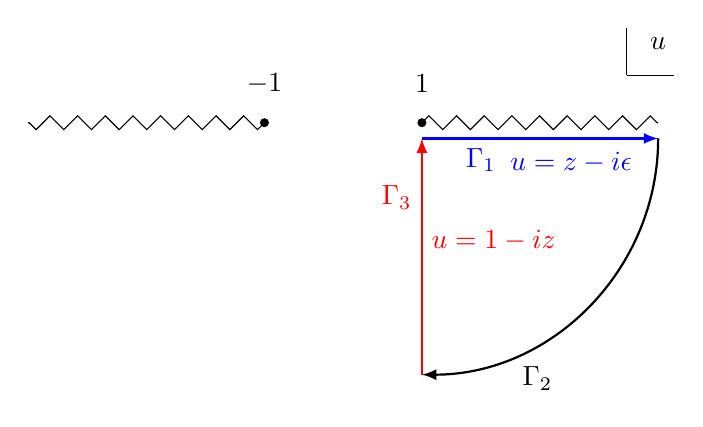
\begin{tikzpicture}
        \node at (4, 1) {$u$};
        \draw (3.6, 0.6) -- (4.2, 0.6);
        \draw (3.6, 0.6) -- (3.6, 1.2);
        \draw[-latex, thick, color=blue] (1,- 0.2) -- (4, -0.2) node[near start, below, color=blue] {$\Gamma_1$};
        \draw[snake=zigzag] (1, 0) -- (4, 0); 
        \draw[snake=zigzag] (-1, 0) -- (-4, 0); 
        \node at (1, 0.5) {$1$};
        \node at (-1, 0.5) {$-1$};
        \node[circle, draw=black, inner sep=1pt, fill=black] at (1, 0) {};
        \node[circle, draw=black, inner sep=1pt, fill=black] at (-1, 0) {};
        \draw[-latex, draw=black, thick] (4, -0.2) arc (0: -90: 3) coordinate (temp1) node[near end, below right] {$\Gamma_2$};
        \draw[-latex, draw=red, thick] (temp1) -- ++(0, 3) node[near end, near end, left, color=red] {$\Gamma_3$};
        \node[color=blue, anchor=west] at (2, -0.5) {$u = z - i\epsilon$};
        \node[color=red, anchor=west] at (1, -1.5) {$u = 1 - iz$};
        
\end{tikzpicture}
\caption{Contour d'intégration pour une séparation de type temps.}
\label{fig:contour2}
\end{figure}

\subsubsection{Amplitude pout le moment conjugué}
On veut évaluer l'amplitude de propagation d'impulsion
\begin{equation}
        D_{\pi}(x - y) = \langle 0 | \hat{\pi}(x) \hat{\pi}(y) | 0 \rangle 
\end{equation} 
On utilise l'expansion de Fourier en terme des opérateurs d'échelle
\begin{align}
        \pi(x) = \int \frac{d^{3}\mathbf{p}}{(2\pi)^{3}}\, e^{-i p \cdot x}\sqrt{\frac{E_{\mathbf{p}}}{2_{\mathbf{p}}}}(a_{\mathbf{p}} - a^{\dagger}_{-\mathbf{p}})\bigg|_{p^{0} = E_{\mathbf{p}}}
\end{align}
pour les opérateurs de moments conjugués. On calcule l'amplitude $D_{\pi}(x - y)$ évaluée sur la coquille d'énergie $p^{0} = E_{\mathbf{p}}$, 
\begin{align*}
D_\pi(x - y) &= \int_{\mathbf{p}} \int_{\mathbf{q}} \frac{\sqrt{E_{\mathbf{p}}E_{\mathbf{q}}}}{2}
        \langle 0 |  (a_{\mathbf{p}}e^{-i p\cdot x} - a^{\dagger}_{\mathbf{p}}e^{i p\cdot x})(a_{\mathbf{q}}e^{-i q \cdot y} - a^{\dagger}_{\mathbf{q}}e^{i q\cdot y})
        | 0 \rangle 
        \bigg|_{\substack{p^{0} = E_{\mathbf{p}} \\ q^{0} = E_{\mathbf{q}}}} \\
        &= -\int_{\mathbf{p}} \int_{\mathbf{q}} \frac{\sqrt{E_{\mathbf{p}}E_{\mathbf{q}}}}{2}
        e^{-i p \cdot x + i q\cdot y}
        \langle 0 | a_{\mathbf{p}}a^{\dagger}_{\mathbf{q}} | 0 \rangle 
        \bigg|_{\substack{p^{0} = E_{\mathbf{p}} \\ q^{0} = E_{\mathbf{q}}}} \\
        &= -\int_{\mathbf{p}}  \frac{E_{\mathbf{p}}}{2}
        e^{-i p \cdot (x - y)}\bigg|_{p^{0} = E_{\mathbf{p}}} 
\end{align*}
On exprime maintenant le quadri-vecteur de séparation dans le système de coordonnées sphériques en suivant les même étapes que précédemment
\begin{align*}
        D_{\pi}(x - y) &=  -\frac{1}{8\pi^2ir}  \int_{-\infty }^{\infty }dp\, p \sqrt{p^2 + m^2}e^{ipr} e^{-i\sqrt{p^2 + m^2}t} 
\end{align*}

\paragraph{Séparation de type espace:} On choisit le contour dans le demi-plan supérieur complexe
\begin{align*}
        D_{\pi}(x - y)
        &= -\frac{1}{4\pi^2r}
        \int_{m }^{\infty } dz\, z \sqrt{z^2 - m^2} e^{-zr}\cosh(\sqrt{z^2 - m^2}t)
\end{align*}
et on choisit un référentiel où $(x - y) = (0, \mathbf{r})$, de sortes que
\begin{align*}
        D_{\pi}(\Lambda(x - y))
        &= -\frac{1}{4\pi^2r}
        \int_{m }^{\infty } dz\, z \sqrt{z^2 - m^2} e^{-zr}
\end{align*}
On fait correspondre cette intégrale avec une fonction de Bessel modifié du second type donnée à l'équation \eqref{eq:bessel2}
avec $t = z / m$
\begin{align*}
        D_{\pi}(\Lambda(x - y)) &= \frac{m^2}{4\pi^2r}\frac{\partial }{\partial r} \int_{1 }^{\infty  } dt\,  \sqrt{t^2 - 1} e^{-mtr} \\
                &= \frac{m^2}{4\pi^2r}\frac{\partial }{\partial r} \left( \frac{2\Gamma(\frac{3}{2})}{\sqrt{\pi} mr} K_1(mr) \right)
\end{align*}
En utilisant le fait que $\Gamma(\frac{3}{2}) = \frac{\sqrt{\pi}}{2}$, on obtient
\begin{align*}
        D_{\pi}(\Lambda(x - y)) &= \frac{m}{4\pi^2r}\frac{\partial }{\partial r} \left( \frac{1}{r} K_1(mr) \right)
\end{align*}
Pour simplifier cette expression, on utilise l'identité \eqref{eq:bessel id1}
\begin{align*}
        D_{\pi}(\Lambda(x - y)) &= \frac{m}{4\pi^2r} \left( -\frac{K_1(mr)}{r^2} - \frac{m}{2r}\big(K_0(mr) + K_2(mr)\big) \right)
\end{align*}
On doit finalement utiliser une une relation de récurrence entre les fonctions de Bessel modifiée de second type qui 
est obtenue à partir d'une de ses fonctions génératives. La relation
\begin{equation}
        K_{\nu}(z) = K_{\nu + 2}(z) - \frac{2(\nu + 1)}{z}K_{\nu + 1}(z)
\end{equation} 
nous permet d'écrire
\begin{align}
        \nonumber
       D_{\pi}(\Lambda(x - y)) &=  -\frac{m}{4\pi^2r} \left( \frac{K_1(mr)}{r^2} + \frac{m}{2r}\big(K_2(mr) - \frac{2}{mr}K_1(mr) + K_2(mr)\big) \right)  \\
        \label{eq:spacelike}
        \implies \Aboxed{D_{\pi}(\Lambda(x - y))  &=  -\frac{m^2}{4\pi^2r^2} K_2(mr)}
\end{align}

\paragraph{Séparation de type temps:} On considère le cas $t > r \geq 0$. On considère d'abord la forme suivante pour l'intégrale, 
qui vient encore une fois d'une étape intermédiaire que j'ai omit puisqu'elle suit des étapes suivit pour $D(x - y)$
\begin{equation}
        D_{\pi}(x - y) = -\frac{1}{4 \pi^2} \int_0^{\infty } dp\, p^2 \frac{\sin(pr)}{pr} \sqrt{p^2 + m^2} e^{-i \sqrt{p^2 + m^2} t}
\end{equation} 
On applique maintenant une transformation de Lorentz tels que $\Lambda(x - y) = (t, \mathbf{0})$, et on applique aussi le changement de variable
\begin{align*}
        u &= \frac{1}{m} \sqrt{p^2 + m^2} \\
       \implies p &=  m\sqrt{u^2 - 1} \\
        du &= \frac{2p dp}{m \sqrt{p^2 + m^2}} = \frac{2p dp}{m^2 u}
\end{align*}
d'où
\begin{align*}
        D_{\pi}(\Lambda(x - y))  &= -\frac{m^4}{8\pi^2} \int_{1}^{\infty } du\, u^2\sqrt{u^2 - 1} e^{-i u mt} \\
                        &= -\frac{m^4}{8\pi^2}\frac{\partial^2}{\partial (mt)^2} \int_{1}^{\infty } du\, \sqrt{u^2 - 1} e^{-i u mt} 
\end{align*}
On répète la procédure faite plus haut pour déterminer cette intégrale, de sortes qu'on obtient
\begin{align*}
       D_{\pi}(\Lambda(x - y)) &= -\frac{im^4}{4\pi} \frac{\partial^2}{\partial (mt)^2} \left( \frac{1}{mt}H^{(2)}_{1}(mt) \right) 
\end{align*}
Pour poursuivre, on introduit les identités
\begin{align}
        \frac{\partial H_{\nu}^{(2)}(z)}{\partial z} &= \frac{1}{2} (H_{\nu  - 1}^{(2)}(z) - H_{\nu + 1}^{(2)}(z)) \\ 
        H_{\nu}^{(2)}(z) &= \frac{2 (\nu + 1)}{z}H_{\nu + 1}^{(2)}(z) - H_{\nu + 2}^{(2)}(z)
\end{align}
qui sont héritées des fonctions de Bessel de premier et second type
\begin{equation}
        H_{\nu}^{(2)} = J_{\nu}(z) - iY_{\nu}(z)
\end{equation} 
En posant $z = mt$, on a
\begin{align*}
        \frac{\partial^{2}}{\partial z^2} \left( \frac{1}{z}H_{1}^{(2)}(z) \right) 
        &= \frac{\partial }{\partial z} \left( 
                - \frac{1}{z^2}H_{1}^{(2)}(z) + \frac{1}{2z} \left( H_{0}^{(2)}(z) - H_{2}^{(2)}(z) \right) 
        \right)\\
        &= \frac{\partial }{\partial z} \left( 
                - \frac{1}{z^2}H_{1}^{(2)}(z) + \frac{1}{2z} \left( \frac{2}{z}H_1^{(2)}(z) - 2H_{2}^{(2)}(z) \right) 
        \right) \\
        &= -\frac{\partial }{\partial z} \left( 
                 \frac{1}{z} H_{2}^{(2)}(z) 
         \right)  \\
         &= -\frac{1}{z^{2}}H_2^{(2)}(z) + \frac{1}{2z} \left( H_1^{(2)}(z) - H_3^{(2)}(z) \right) \\
         &= -\frac{1}{z^{2}}H_2^{(2)}(z) + \frac{1}{2z} \left( \frac{4}{z}H_{2}^{(2)}(z) - 2H_3^{(2)}(z) \right) \\
         &= -\frac{1}{z} \left( \frac{1}{z} H_2^{(2)}(z) - H_{3}^{(2)}(z) \right) \\
         &= -\frac{1}{z}\bigg(H_{1}^{(2)}(z) - \frac{1}{z}H_2^{(2)}\bigg)
\end{align*}
On obtient finalement
\begin{equation}
        \boxed{D_{\pi}(\Lambda(x - y)) = \frac{im^3}{4\pi t} \left( H_{1}^{(2)}(mt) - \frac{1}{mt}H_{2}^{(2)}(mt) \right) }
\end{equation} 
De façon générale
\begin{equation}
        \boxed{
        D_{\pi}(x - y) = \begin{cases}
                -\dfrac{m^2}{4\pi^2r^2} K_2(mr),  & (x - y)^{2} < 0, \hspace{0.5cm} \Lambda(x - y) = (0, \mathbf{r}) \\[2ex]
                 \dfrac{im^3}{4\pi t} \left( H_{1}^{(2)}(mt) - \dfrac{1}{mt}H_{2}^{(2)}(mt) \right),  & (x - y)^{2} > 0, \hspace{0.5cm} \Lambda(x - y) = (t, \mathbf{0})
        \end{cases}
}
\end{equation} 


\subsection{}
On applique la transformation d'échelle au propagateur de position, de sortes que
\begin{equation}
        D(x' - y') = \langle 0 | \hat{\phi}'(x') \hat{\phi}'(y') | 0 \rangle 
\end{equation} 
On cherche le facteur d'échelle $\Delta$, et on veut comparer avec le devoir 1.

\subsection{}
%En évaluant $D$ pour des temps égaux, que pouvez-vous conclure à propos de l’étendue
%spatiale de l’état $\hat{\phi}(x) | 0 \rangle $ ?\\

Dans la figure \ref{fig:amplitudes}, on évalue numériquement les différentes amplitudes calculées dans ce numéro. On remarque 
que la taille caractéristique de la courbe rouge, soit l'amplitude calculée à temps égal, est $r = \frac{1}{m}$. 
J'interprète la taille caractéristique comme la distance $r$ où l'amplitude de genre espace accomplit un premier pliage exponentielle.
Évidemment, on peut aussi déterminer ceci par une analyse asymptotique de $D(x - y) \sim e^{-mr}$, d'où on aurait 
pu deviner ce comportement.

De façon intéressante, cela correspond à la longueur d'onde de Compton (dans le système d'unité naturelles).
On peut donc supposer que l'étendue spatiale de $\phi(x) | 0 \rangle $ est de l'ordre de $\frac{1}{\sqrt{m}}$ dans la théorie 
de Klein-Gordon.
%Physiquement, on interprète cette distance comme la région de l'espace
\begin{figure}
        \centering
        \includegraphics[width=0.8\textwidth]{amplitudes.pdf}
        \caption{Amplitudes évaluée avec $m=1$, sur l'interval $[0.1, 10]$.}
        \label{fig:amplitudes}
\end{figure}



\section{Opérateur de nombre}

\subsection{}
Soit l’opérateur $\hat{n}_{\mathbf{p}} = \hat{a}^{\dagger}_{\mathbf{p}}\hat{a}_{\mathbf{p}}$. 
En premier lieu, on cherche à savoir si cet opérateur commute avec l’Hamiltonien de Klein-Gordon. \\
\begin{align*}
        [\hat{n}_{\mathbf{p}}, \hat{H}] &=  \int_{\mathbf{q}}E_{\mathbf{q}}[\hat{a}^{\dagger}_{\mathbf{p}}\hat{a}_{\mathbf{p}}, \hat{a}^{\dagger}_{\mathbf{q}}\hat{a}_{\mathbf{q}}] \\
                                        &= \int_{\mathbf{q}} E_\mathbf{q} \big(\hat{a}^{\dagger}_{\mathbf{q}}[\hat{a}^{\dagger}_{\mathbf{p}},\, \hat{a}_{\mathbf{q}}]\hat{a}_{\mathbf{p}} 
                                        + \hat{a}^{\dagger}_{\mathbf{q}}[\hat{a}_{\mathbf{p}},\, \hat{a}^{\dagger}_{\mathbf{q}}]\hat{a}_{\mathbf{p}} \big) \\
                                        &= \int_{\mathbf{q}} E_\mathbf{q} \big(-\hat{a}^{\dagger}_{\mathbf{q}}\hat{a}_{\mathbf{p}} 
                                        + \hat{a}^{\dagger}_{\mathbf{q}}\hat{a}_{\mathbf{p}} 
                                        \big) 
                                        (2\pi)^{m}\delta^{(n)}(\mathbf{p} - \mathbf{q}) \\
                                        &= 0
\end{align*}
Donc, \textbf{l'opérateur $\hat{n}_{\mathbf{q}}$ commute avec l'Hamiltonien}. Dans ce cas, 
l'évolution temporelle de $\hat{n}_{\mathbf{q}}$ est $\frac{d}{dt} \hat{n}_{\mathbf{q}} = i[\hat{H}, \hat{n}] = 0$, 
donc
\textbf{l'opérateur $\hat{n}_{\mathbf{q}}$ n'évolue pas dans le temps}. On conclue que le nombre de 
particules dans un état d'énergie $E_{\mathbf{p}}$ est constant dans le temps. L'énergie total des particules 
d'impulsion $\mathbf{p}$, $E_{\mathbf{p}}$, est conservée. 

\subsection{}
On s'intéresse à l'action de $\hat{n}_{\mathbf{q}}$ sur les états $| 0 \rangle$, $| p \rangle $ et $|p, p' \rangle $, sans se soucier 
de la normalisation des états. Autrement, on pose $| p \rangle  = a^{\dagger}_{\mathbf{p}} | 0 \rangle $.
Pour l'état fondamental, on a
\begin{equation}
        \hat{n}_{\mathbf{q}}| 0 \rangle  = a^{\dagger}_{\mathbf{q}} \hat{a}_{\mathbf{q}} | 0 \rangle = 0
\end{equation} 
Pour l'état d'une seule particule, on a
\begin{align*}
        \hat{n}_{q} | p \rangle &=  \hat{n}_{\mathbf{q}} \hat{a}^{\dagger}_{\mathbf{p}} | 0 \rangle  \\
                        &= \hat{a}^{\dagger}_{\mathbf{q}} \hat{a}_{\mathbf{q}} \hat{a}^{\dagger}_{\mathbf{p}} | 0 \rangle \\
                        &= \hat{a}^{\dagger}_{\mathbf{q}}[\hat{a}_{\mathbf{q}}, \hat{a}^{\dagger}_{\mathbf{p}}] | 0 \rangle \\
                        &= (2\pi)^{d}\delta^{(n)}(\mathbf{p} - \mathbf{q})\hat{a}^{\dagger}_{\mathbf{q}} | 0 \rangle \\
                        &= (2\pi)^{d}\delta^{(n)}(\mathbf{p} - \mathbf{q})| q \rangle 
\end{align*}
%On trouve que dans le cas où $\mathbf{p} = \mathbf{q}$, une intégrale sur l'espace de phase va recouvrir l'état $| p \rangle $, avec une valeur propre $N_{\mathbf{p}} = 1$.
Pour l'état avec 2 particules, on a
\begin{align*}
        \hat{n}_{\mathbf{q}} | p, p' \rangle  &= \hat{a}^{\dagger}_{\mathbf{q}} \hat{a}_{\mathbf{q}} \hat{a}^{\dagger}_{\mathbf{p}}\hat{a}^{\dagger}_{\mathbf{p}'} | 0 \rangle  \\
        &= \hat{a}^{\dagger}_{\mathbf{q}} \hat{a}^{\dagger}_{\mathbf{p}}\hat{a}_{\mathbf{q}} \hat{a}^{\dagger}_{\mathbf{p}'} | 0 \rangle 
        + \hat{a}^{\dagger}_{\mathbf{q}}[ \hat{a}_{\mathbf{q}}, \hat{a}^{\dagger}_{\mathbf{p}}]\hat{a}^{\dagger}_{\mathbf{p}'} | 0 \rangle  \\
        &= \hat{a}^{\dagger}_{\mathbf{q}} \hat{a}^{\dagger}_{\mathbf{p}}[\hat{a}_{\mathbf{q}}, \hat{a}^{\dagger}_{\mathbf{p}'}] | 0 \rangle 
        + \hat{a}^{\dagger}_{\mathbf{q}}[ \hat{a}_{\mathbf{q}}, \hat{a}^{\dagger}_{\mathbf{p}}]\hat{a}^{\dagger}_{\mathbf{p}'} | 0 \rangle  \\
        &= (2\pi)^{d}\delta^{(n)}(\mathbf{q} - \mathbf{p}')\hat{a}^{\dagger}_{\mathbf{q}} \hat{a}^{\dagger}_{\mathbf{p}}| 0 \rangle 
        + (2\pi)^{d}\delta^{(n)}(\mathbf{q} - \mathbf{p})\hat{a}^{\dagger}_{\mathbf{q}}\hat{a}^{\dagger}_{\mathbf{p}'} | 0 \rangle  \\
        &= (2\pi)^{d}\delta^{(n)}(\mathbf{q} - \mathbf{p}')| p, q \rangle 
        + (2\pi)^{d}\delta^{(n)}(\mathbf{q} - \mathbf{p})| p', q \rangle  \\
\end{align*}
%Dans le cas où $\mathbf{p} = \mathbf{p}' = \mathbf{q}$, on trouve un état avec 2 particules. 
%Autrement dit, le nombre d'état avec le niveau d'énergie 
%$E_{\mathbf{p}}$ sont comptées.

\subsection{}
On définit l'opérateur nombre 
\begin{equation}
        \hat{N} = \int \frac{d^{d}\mathbf{p}}{(2\pi)^{d}} \hat{n}_{\mathbf{p}}
\end{equation} 
Les valeurs propres de cet opérateurs sont données par le nombre total de particules dans un état. Par exemple,
\begin{align*}
        \hat{N} | p_1 \dots p_n \rangle &= \int_{\mathbf{q}} \hat{n}_{\mathbf{q}} a^{\dagger}_{\mathbf{p}_1} \dots a^{\dagger}_{\mathbf{p}_n} | 0 \rangle  \\
        &= \int_{\mathbf{q}} \sum_{i=1}^{n} (2\pi)^{d}\delta^{(n)}(\mathbf{q} - \mathbf{p}_i) | p_1 \dots p_n \rangle  \\
        &= n | p_1 \dots p_n \rangle 
\end{align*}
Les vecteurs propres de cet opérateurs sont donc tous les états de l'espace de Fock. 


\subsection{}
L'opérateur de nombre $\hat{N}$ commute avec l'Hamiltonien 
\begin{align*}
        [\hat{N}, \hat{H}] = \int_{\mathbf{p}}  [\hat{n}_{\mathbf{p}}, \hat{H}] = 0
\end{align*}
Dans ce cas, $\frac{d}{dt}\hat{N} = -i[\hat{N}, \hat{H}] = 0$, l'opérateur de nombre est une constante temporelle dans la théorie de Klein-Gordon. Donc le nombre de 
particules total dans un système est préservée.
Ceci revient à dire que \textbf{l'énergie totale est conservée}.

\subsection{}
On ajoute maintenant un terme d'intéraction $\lambda \phi^{4}$ à l'Hamiltonien. 

\section{Le champ scalaire complexe}
On considère l'action de Klein-Gordon pour un opérateur de champ complexe $\phi$
\begin{equation}
        S = \int d^{4}x\, \partial_{\mu} \phi^{\dagger} \partial^{\mu}\phi - m^{2} \phi^{\dagger}\phi
\end{equation} 

\subsection{}
On s'intéresse aux moments conjugués de $\phi$ et $\phi^{\dagger}$. Par définition
\begin{align}
        \pi &=  \frac{\partial \mathcal{L}}{\partial \dot{\phi}} = \frac{\partial }{\partial (\partial_0 \phi)} (\partial_\mu \phi^{\dagger} \partial^{\mu} \phi - m^{2} \phi^{\dagger}\phi) \\
        \implies \pi &=  \dot{\phi}^{\dagger}
\end{align}
De la même façon, on trouve
\begin{equation}
        \pi^{\dagger} = \dot{\phi}
\end{equation} 
Les relations de commutations canoniques, à temps égal, sont
\begin{align}
        [\phi(\mathbf{x}, t), \pi(\mathbf{y}, t)] &= [\phi^{\dagger}(\mathbf{x}, t), \pi^{\dagger}(\mathbf{y}, t)] = i\delta^{(3)}(\mathbf{x} - \mathbf{y})
\end{align}
Toute les autres relations sont nulles. L'Hamiltonien est la transformée de Legendre du Lagrangien, d'où
\begin{equation}
        H = \int d^3\mathbf{x}\, (\pi \dot{\phi} + \pi^{\dagger} \dot{\phi}^{\dagger} - \mathcal{L}) = \int d^{3}\mathbf{x}\, (\pi^{\dagger}\pi + \grad \phi^{\dagger} \grad \phi + m^{2} \phi^{\dagger} \phi)
\end{equation} 
Finalement, on calcule les équations de mouvement selon le point de vue de Heisenberg, $\frac{\partial \hat{A}}{\partial t} = -i[\hat{A}, H]$. 
Puisque $H$ est une charge de Noether, $\frac{dH}{dt} = 0$ lorsque les équations de mouvement sont respectée. 
Dans ce cas, on peut évaluer $H$ à n'importe quel temps $t$. En particulier, 
on choisit de l'évaluer au même temps que l'opérateur qu'il fait évoluer. Pour l'opérateur de champ $\phi$, on trouve l'équation de mouvement 
\begin{align*}
        \dot{\phi}(\mathbf{x}, t) &= -i[\phi(\mathbf{x}, t),\, H] \\
        &= -i\int d^{3}\mathbf{y}\, 
        \left[ 
                \phi(\mathbf{x}, t),\,
                \pi^{\dagger}(\mathbf{y}, t) \pi(\mathbf{y},t)
                + \grad \phi^{\dagger}(\mathbf{y}, t) \grad \phi(\mathbf{y}, t) 
                + m^2 \phi^{\dagger}(\mathbf{y}, t) \phi(\mathbf{y}, t)
        \right] \\
        &= -i\int d^{3}\mathbf{y}\, \pi^{\dagger}(\mathbf{y}, t)[\phi(\mathbf{x}, t),\, \pi(\mathbf{y}, t)] \\
        &= -i \int d^{3}\mathbf{y}\, \pi^{\dagger}(\mathbf{y}, t) i \delta^{(3)}(\mathbf{x} - \mathbf{y}) \\
        &= \pi^{\dagger}(\mathbf{x}, t)
\end{align*}
Ce qui est bien le résultat attendu. Pour le champ conjugué, on a l'équation d'évolution $\dot{\phi}^{\dagger}(\mathbf{x}, t) = \pi(\mathbf{x}, t)$ par 
un argument similaire. On s'intéresse maintenant à l'équation de mouvement du moment conjugué $\pi$:
\begingroup
\allowdisplaybreaks
\begin{align*}
        \dot{\pi}(\mathbf{x}, t) &= -i[\pi(\mathbf{x}, t), \, H] \\
                &= -i \int d^{3}\mathbf{y}\, 
        [\pi(\mathbf{x}, t),\, 
                \pi^{\dagger}(\mathbf{y}, t) \pi(\mathbf{y},t)
                + \grad \phi^{\dagger}(\mathbf{y}, t) \grad \phi(\mathbf{y}, t) 
                + m^2 \phi^{\dagger}(\mathbf{y}, t) \phi(\mathbf{y}, t)
        ]\\
        &= -i \int d^{3}\mathbf{y}\,
        \bigg(  
        \grad \phi^{\dagger}(\mathbf{y}, t)
        [\pi(\mathbf{x}, t),\, \grad \phi(\mathbf{y}, t)]
        + m^2 \phi^{\dagger}(\mathbf{y}, t) [\pi(\mathbf{x}, t),\, \phi(\mathbf{y}, t)] 
        \bigg)\\
        &= -i \int d^{3}\mathbf{y}\, \bigg( 
        \grad \phi^{\dagger}(\mathbf{y}, t) (-i\grad\delta^{(3)}(\mathbf{x} - \mathbf{y})) + m^2 \phi^{\dagger}(\mathbf{y}, t)(-i \delta^{(3)}(\mathbf{x} - \mathbf{y}))
        \bigg)
\end{align*}
\endgroup
Le premier terme de cette expression est écrit en terme de gradient d'une fonction delta de Dirac. Pour progresser, on intègre par partie 
ce premier terme sachant que $\int_u\, f(u) \grad \delta(u - x) = -\grad f(x)$, de sortes que
\begin{align*}
         \implies \dot{\pi}(\mathbf{x}, t) &= 
         \grad^2 \phi^{\dagger}(\mathbf{x}, t) - m^2 \phi^{\dagger}(\mathbf{x}, t)     
\end{align*}
On obtient $\dot{\pi}^{\dagger}(\mathbf{x}, t) = \grad^{2} \phi(\mathbf{x}, t) - m^{2}\phi(\mathbf{x}, t)$ par des arguments similaires. Finalement, on
obtient les équations de mouvements le champ $\phi$:
\begin{equation}
        \partial_t^{2} \phi = \partial_t \pi^{\dagger} = \grad^{2}\phi - m^{2} \phi
\end{equation} 
En collectant les terme, on trouve bien l'équation de mouvement de Klein-Gordon
\begin{equation}
        (\partial_t^2 - \grad^2 + m^2) \phi = 0
\end{equation} 

\subsection{}

On cherche maintenant à diagonaliser l'Hamiltonien, et on cherche aussi à montrer qu'il contient deux ensembles de particules, chacune de masse $m$.  
Je m'intéresse d'abord au second objectif.
On commence par découpler les champs $\phi$ et $\pi$ en 
terme d'une superposition de deux champs réels
\begin{align}
        \phi &= \frac{1}{\sqrt{2}}(\phi_1 + i\phi_2) \\
        \pi &= \frac{1}{\sqrt{2}}(\pi_1 - i \pi_2)
\end{align}
Le signe moins pour le moment conjugué est placé en anticipation de ce qui va suivre.
En inversant ces relations,  on trouve
\begin{equation}
        \begin{matrix}
                \phi_1 = \dfrac{1}{\sqrt{2}}(\phi + \phi^{\dagger})\, &\hspace{.5cm} \phi_2 = -\dfrac{i}{\sqrt{2}}(\phi - \phi^{\dagger}) \\[3ex]
                \pi_1 = \dfrac{1}{\sqrt{2}}(\pi + \pi^{\dagger})\, &\hspace{.5cm} \pi_2 = \dfrac{i}{\sqrt{2}}(\pi - \pi^{\dagger})
        \end{matrix}
\end{equation} 
On peut maintenant déduire les relations de commutations de ces champs réels en utilisant les relations canoniques pour $\phi$ et $\pi$. On a
\begin{align*}
        [\phi_1(\mathbf{x}, t), \pi_1(\mathbf{y}, t)] &= \frac{1}{2}[\phi(\mathbf{x}, t) + \phi^{\dagger}(\mathbf{x}, t),\, \pi(\mathbf{y}, t) + \pi^{\dagger}(\mathbf{y}, t)] \\
                        &= \frac{1}{2}[\phi(\mathbf{x}, t), \pi(\mathbf{x}, t)] + \frac{1}{2}[\phi^{\dagger}(\mathbf{x}, t), \pi^{\dagger}(\mathbf{x}, t)] \\
                        &= i \delta^{(3)}(\mathbf{x} - \mathbf{y})
\end{align*}
et
\begin{align*}
        [\phi_2(\mathbf{x}, t), \pi_2(\mathbf{y}, t)] &= \frac{1}{2}[\phi(\mathbf{x}, t) - \phi^{\dagger}(\mathbf{x}, t),\, \pi(\mathbf{y}, t) - \pi^{\dagger}(\mathbf{y}, t)] \\
                        &= \frac{1}{2}[\phi(\mathbf{x}, t), \pi(\mathbf{x}, t)] + \frac{1}{2}[\phi^{\dagger}(\mathbf{x}, t), \pi^{\dagger}(\mathbf{x}, t)] \\
                        &= i \delta^{(3)}(\mathbf{x} - \mathbf{y})
\end{align*}
On peut écrire de façon compacte 
\begin{equation}
        [\phi_i(\mathbf{x}, t), \pi_j(\mathbf{y}, t)] = i \delta_{ij} \delta^{(3)}(\mathbf{x} - \mathbf{y})
\end{equation} 
Les autres relations sont trivialement nulles. Avec ces relations, on observe que les produits scalaires $\phi^{\dagger}\phi$ et $\pi^{\dagger}\pi$ se simplifient en deux termes 
découplés. Par exemple
\begin{align*}
        \phi^{\dagger} \phi &=  (\phi_1 - i\phi_2)(\phi_1 + i \phi_2) \\
        &= \phi_1^2 + \phi_2^2 - i\phi_2\phi_1 + i\phi_1 \phi_2 \\
        &= \phi_1^2 + \phi_2^2 + i[\phi_1, \phi_2] \\
        &= \phi_1^2 + \phi_2^2
\end{align*}
On obtient finalement deux Hamiltoniens découplés
\begin{align*}
        H &= \frac{1}{2}\int d^{3}\mathbf{x}\, \bigg(\pi^{\dagger}\pi + \grad \phi^{\dagger} \grad \phi + m^{2} \phi^{\dagger}\phi \bigg) \\
        &= \frac{1}{2} \int d^{3}\mathbf{x}\, \bigg( \pi_1^{2} + \pi_2^{2} + (\grad \phi_1)^2 + (\grad \phi_2)^2 + m^{2}\phi_1^2 + m^2 \phi_2^2  \bigg) \\
        &= H_1 + H_2
\end{align*}
\textbf{La théorie du champ scalaire complexe contient donc deux particules de masses $m$.}

On peut maintenant diagonaliser ces Hamiltoniens par une expansion des champs en terme de leur modes de Fourier. 
On introduit deux opérateurs d'échelles, $a_{\mathbf{p}}$ et $b_{\mathbf{p}}$, soit un 
opérateur d'échelle pour chaque Hamiltonien. Par correspondance avec les opérateurs d'échelles classiques, on a
\begin{align}
        \phi_1(\mathbf{x}) &=  \int \frac{d^{3}\mathbf{p}}{(2 \pi)^{3}}e^{i \mathbf{p} \cdot \mathbf{x}} \frac{1}{\sqrt{2 E_{\mathbf{p}}}} (a_{\mathbf{p}} + a^{\dagger}_{-\mathbf{p}}) \\
        \pi_1(\mathbf{x}) &=  \int \frac{d^{3}\mathbf{p}}{(2 \pi)^{3}} e^{i \mathbf{p} \cdot \mathbf{x}} (-i)\sqrt{\frac{E_{\mathbf{p}}}{2}}(a_{\mathbf{p}} - a^{\dagger}_{-\mathbf{p}}) \\
        \phi_2(\mathbf{x}) &=  \int \frac{d^{3} \mathbf{x}}{(2\pi)^{3}}e^{i\mathbf{p} \cdot \mathbf{x}}\frac{1}{\sqrt{2E_{\mathbf{p}}}} (b_{\mathbf{p}} + b^{\dagger}_{-\mathbf{p}}) \\
        \pi_2(\mathbf{x}) &=  \int \frac{d^{3}\mathbf{p}}{(2 \pi)^{3}} e^{i \mathbf{p} \cdot \mathbf{x}} (-i)\sqrt{\frac{E_{\mathbf{p}}}{2}}(b_{\mathbf{p}} - b^{\dagger}_{-\mathbf{p}}) \\
\end{align} 
On a introduit l'énergie d'une particule avec une quantité de mouvement $\mathbf{p}$ 
et de masse $m$:
\begin{equation}
        E_{\mathbf{p}} = \sqrt{\mathbf{p}^2 + m^2}
\end{equation} 
Avec ces expansions de Fourier, on obtient deux Hamiltoniens qui correspondent à un oscillateur harmonique simple. Leur somme est donc
\begin{equation}
        H = \int \frac{d^{3}\mathbf{p}}{(2\pi)^{3}}\, E_{\mathbf{p}}(a^{\dagger}_{\mathbf{p}}a_{\mathbf{p}} + b^{\dagger}_{\mathbf{p}}b_{\mathbf{p}})
\end{equation} 
Je finis ce problème en montrant que l'expansion de Fourier des champs complexes $\phi$ et $\pi$ peut être construite en terme 
des opérateurs d'échelles que j'ai introduit pour les champs réels. 
%Il est maintenant trivial de montrer que le problème peut se faire en commençant 
%avec la prochain équation (la méthode préférée par Peskins et Schroeder). Toutefois, je considère cette approche beaucoup moins intuitive. 
On introduit deux opérateurs d'échelles mixtes, soit
\begin{align}
        \label{eq:A mixte}
        A_{\mathbf{p}} &= \frac{1}{\sqrt{2}}(a_{\mathbf{p}} + ib_{\mathbf{p}}) \\
        \label{eq:B mixte}
        B_{\mathbf{p}} &=  \frac{1}{\sqrt{2}}(a_{\mathbf{p}} - ib_{\mathbf{p}})
\end{align}
De sortes que
\begin{align}
        \nonumber
        \phi(\mathbf{x}) &=  \frac{1}{\sqrt{2}}\int \frac{d^{3}\mathbf{p}}{(2 \pi)^{3}} e^{i \mathbf{p} \cdot \mathbf{x}} \frac{1}{\sqrt{2 E_{\mathbf{p}}}} 
        (a_{\mathbf{p}} + a^{\dagger}_{-\mathbf{p}} + ib_{\mathbf{p}} + i\mathbf{b}^{\dagger}_{-\mathbf{p}})  \\
        \label{eq:phi AB}
        &= \int \frac{d^{3} \mathbf{p}}{(2\pi)^{3}} e^{i \mathbf{p} \cdot \mathbf{x}} \frac{1}{\sqrt{2 E_{\mathbf{p}}}} (A_{\mathbf{p}} + B^{\dagger}_{-\mathbf{p}})
\end{align}
et
\begin{align}
        \nonumber
        \pi(\mathbf{x}) &=  \frac{1}{\sqrt{2}}\int \frac{d^{3}\mathbf{p}}{(2 \pi)^{3}} e^{i \mathbf{p} \cdot \mathbf{x}} (-i)\sqrt{\frac{E_{\mathbf{p}}}{2 }} 
        (a_{\mathbf{p}} - a^{\dagger}_{-\mathbf{p}} - i(b_{\mathbf{p}} - \mathbf{b}^{\dagger}_{-\mathbf{p}}))  \\
        \label{eq:pi AB}
        &=  \int \frac{d^{3}\mathbf{p}}{(2 \pi)^{3}} e^{i \mathbf{p} \cdot \mathbf{x}} (-i)\sqrt{\frac{E_{\mathbf{p}}}{2 }} 
        (B_{\mathbf{p}} - A^{\dagger}_{-\mathbf{p}}) 
\end{align}
Notons que l'Hamiltonien se sépare trivialement en terme de $A_{\mathbf{p}}$ et $B_{\mathbf{p}}$. Cette observation suit de leur relation de commutation. 
On peut déduire ces relations à partir des relations de commutations canoniques respectées par $a_{\mathbf{p}}$ et $b_{\mathbf{p}}$. En particulier
\begin{align*}
        [A_{\mathbf{p}}, A^{\dagger}_{\mathbf{q}}] &= \frac{1}{2}[a_{\mathbf{p}} + ib_{\mathbf{p}}, a^{\dagger}_{\mathbf{q}} - ib^{\dagger}_{\mathbf{q}}] \\
                                                   &= \frac{1}{2}([a_{\mathbf{p}}, a^{\dagger}_{\mathbf{q}}] - i^2[b_{\mathbf{p}}, b^{\dagger}_{\mathbf{q}}]) \\
                                                   &= (2\pi)^{3} \delta^{(3)}(\mathbf{p} - \mathbf{q})
\end{align*}
et
\begin{align*}
        [B_{\mathbf{p}}, B^{\dagger}_{\mathbf{q}}] &= \frac{1}{2}[a_{\mathbf{p}} - ib_{\mathbf{p}}, a^{\dagger}_{\mathbf{q}} + ib^{\dagger}_{\mathbf{q}}] \\
                                                   &= \frac{1}{2}([a_{\mathbf{p}}, a^{\dagger}_{\mathbf{q}}] - i^2[b_{\mathbf{p}}, b^{\dagger}_{\mathbf{q}}]) \\
                                                   &= (2\pi)^{3} \delta^{(3)}(\mathbf{p} - \mathbf{q})
\end{align*}
Les opérateurs d'échelles $A_{\mathbf{p}}$ et $B_{\mathbf{p}}$ respectent donc eux aussi les relations de commutations canoniques. 
Ainsi, en soustrayant le delta de Dirac de l'Hamiltonien et en utilisant l'ordre normal des modes, on inverse les relations 
\eqref{eq:A mixte} et \eqref{eq:B mixte} pour obtenir
\begin{equation}
        H = \int \frac{d^{3}\mathbf{p}}{(2\pi)^{3}} E_{\mathbf{p}}(A^{\dagger}_\mathbf{p}A_{\mathbf{p}} + B^{\dagger}_{\mathbf{p}}B_{\mathbf{p}})
\end{equation} 


\subsection{}
On considère la charge de Noether
\begin{equation}
        Q = i\int d^{3}\mathbf{x}\, (\phi^{\dagger}\pi^{\dagger} - \pi \phi)
\end{equation} 
On cherche à réécrire cette charge en terme des opérateurs d'échelles $A_{\mathbf{p}}$ et $B_{\mathbf{p}}$. On applique les expansions en modes 
de Fourier \eqref{eq:phi AB} et \eqref{eq:pi AB}, de sortes que
\begin{align*}
        Q &=  
        -\int d^{3}\mathbf{x}\, \bigg(  
\int_{\mathbf{p}}e^{-i \mathbf{p} \cdot \mathbf{x}} \frac{1}{\sqrt{2 E_{\mathbf{p}}}} (A^{\dagger}_{\mathbf{p}} + B_{-\mathbf{p}})
\int_{\mathbf{q}} e^{-i \mathbf{q} \cdot \mathbf{x}} \sqrt{\frac{E_{\mathbf{q}}}{2 }} (B^{\dagger}_{\mathbf{q}} - A_{-\mathbf{q}}) \\
          &\hspace{2cm}+ 
\int_{\mathbf{p}}e^{i \mathbf{p} \cdot \mathbf{x}} \frac{1}{\sqrt{2 E_{\mathbf{p}}}} (A_{\mathbf{p}} + B^{\dagger}_{-\mathbf{p}})
\int_{\mathbf{q}} e^{i \mathbf{q} \cdot \mathbf{x}} \sqrt{\frac{E_{\mathbf{q}}}{2 }} (B_{\mathbf{q}} - A^{\dagger}_{-\mathbf{q}}) 
\bigg)  \\
&= 
        -\frac{1}{2}\int d^{3}\mathbf{x}\, \bigg(  
\int_{\mathbf{p}} \int_{\mathbf{q}} e^{-i (\mathbf{p} + \mathbf{q}) \cdot \mathbf{x}} \sqrt{\frac{E_{\mathbf{q}}}{ E_{\mathbf{p}}}} 
(A^{\dagger}_{\mathbf{p}} + B_{-\mathbf{p}})(B^{\dagger}_{\mathbf{q}} - A_{-\mathbf{q}}) \\
          &\hspace{2cm}+ 
\int_{\mathbf{q}} \int_{\mathbf{p}} e^{i(\mathbf{q} + \mathbf{p}) \cdot \mathbf{x}} \sqrt{\frac{E_{\mathbf{q}}}{E_{\mathbf{p}} }} 
 (A_{\mathbf{p}} + B^{\dagger}_{-\mathbf{p}})(B_{\mathbf{q}} - A^{\dagger}_{-\mathbf{q}})\bigg)  \\
&= 
        -\frac{1}{2} \bigg(  
                \int_{\mathbf{p}} \int_{\mathbf{q}} (2\pi)^{3}\delta^{(3)}(\mathbf{p} + \mathbf{q}) \sqrt{\frac{E_{\mathbf{q}}}{ E_{\mathbf{p}}}} 
(A^{\dagger}_{\mathbf{p}} + B_{-\mathbf{p}})(B^{\dagger}_{\mathbf{q}} - A_{-\mathbf{q}}) \\
          &\hspace{1cm}+ 
          \int_{\mathbf{q}} \int_{\mathbf{p}} (2\pi)^{3}\delta^{(3)}(\mathbf{p} + \mathbf{q})  \sqrt{\frac{E_{\mathbf{q}}}{E_{\mathbf{q}} }}
 (A_{\mathbf{p}} + B^{\dagger}_{-\mathbf{p}})(B_{\mathbf{q}} - A^{\dagger}_{-\mathbf{q}})\bigg)  \\
\end{align*}
Où on a appliqué la définition de la fonction delta de Dirac. En appliquant le delta de Dirac, on obtient une 
somme de produits d'opérateurs d'échelles. Par inspection, on va trouver que les termes mixtes s'annulent entre eux, ce qui 
suit de leur relation de commutation. En effet,
\begin{align*}
Q        
&= 
-\frac{1}{2} 
                \int_{\mathbf{p}} \big((A^{\dagger}_{\mathbf{p}} + B_{-\mathbf{p}})(B^{\dagger}_{-\mathbf{p}} - A_{\mathbf{p}}) 
                + (A_{\mathbf{p}} + B^{\dagger}_{-\mathbf{p}})(B_{-\mathbf{p}} - A^{\dagger}_{\mathbf{p}}) \big) \\
&= 
        -\frac{1}{2} 
        \int_{\mathbf{p}} \big(-A^{\dagger}_{\mathbf{p}}A_{\mathbf{p}} - A_{\mathbf{p}}A^{\dagger}_{\mathbf{p}} + B_{-\mathbf{p}}B^{\dagger}_{-\mathbf{p}} + B^{\dagger}_{-\mathbf{p}}B_{-\mathbf{p}} + [A^{\dagger}_{\mathbf{p}}, B^{\dagger}_{-\mathbf{p}}] + [B_{-\mathbf{p}}, A_{\mathbf{p}}])
\end{align*}
Puisque $[A^{\dagger}_{\mathbf{p}}, B^{\dagger}_{-\mathbf{p}}] = [B_{-\mathbf{p}}, A_{\mathbf{p}}] = 0$, on obtient
\begin{equation}
        Q =  \int \frac{d^{3}\mathbf{p}}{(2 \pi)^{3}} ( A^{\dagger}_{\mathbf{p}}A_{\mathbf{p}} - B^{\dagger}_{\mathbf{p}}B_{\mathbf{p}} 
        + [A_{\mathbf{p}}, A^{\dagger}_{\mathbf{p}}] - [B_{\mathbf{p}}, B^{\dagger}_{\mathbf{p}}])
\end{equation} 
où on a pris la liberté de redéfinir la variable $-\mathbf{p} \rightarrow \mathbf{p}$ pour l'opérateur $B_{-\mathbf{p}}$, ce qui ne change 
pas le résultat de l'intégral sur tout l'espace de phase. Finalement, on remarque que les deux 
commutateurs restants s'annulent entre eux, et on obtient
\begin{equation}
        \boxed{Q = \int \frac{d^{3}\mathbf{p}}{(2 \pi)^{3}} (A^{\dagger}_{\mathbf{p}}A_{\mathbf{p}} - B^{\dagger}_{\mathbf{p}}B_{\mathbf{p}})}
\end{equation} 
En examinant les commutateurs entre la charge et les opérateurs de créations, 
\begin{align}
        [Q, A^{\dagger}_{\mathbf{p}}] &= \int_{\mathbf{q}} A^{\dagger}_{\mathbf{q}}[A_{\mathbf{p}}, A^{\dagger}_{\mathbf{p}}] = A^{\dagger}_{\mathbf{p}} \\
        [Q, B_{\mathbf{p}}^{\dagger}] &= - \int_{\mathbf{q}} B^{\dagger}_{\mathbf{q}}[B_{\mathbf{q}}, B^{\dagger}_{\mathbf{p}}] = -B^{\dagger}_{\mathbf{p}}
\end{align} 
on constate que la particule associée à $A^{\dagger}_{\mathbf{p}}$ possède une charge positive et la particule associée à 
$B^{\dagger}_{\mathbf{p}}$ possède une charge négative.

\subsection{}
On considère deux champs de Klein-Gordon complexe, $\phi_a(\mathbf{x}, t)$, $a \in \{1, 2\}$, avec la même masse $m$.
Le Lagrangien est maintenant
\begin{equation}
        \mathcal{L} = \partial_{\mu} \phi_a^{\dagger} \partial^{\mu}\phi_a - m^{2} \phi_a^{\dagger}\phi_a
\end{equation} 
%Ce Lagrangien, comme le précédent, possède une symétrie de phase, ç.-à-d. une transformation du group $U(1)$
%Toutefois, 
Ce Lagrangien possède une symétrie $U(2)$, soit un isomorphisme à $SU(2) \times U(1)$, où $U(1)$ est une symétrie de 
phase ($U(1) = \{z \mid z \in \mathbb{C}, |z| = 1\}$, soit le cercle unité)
\begin{align*}
        \phi_a &\rightarrow e^{-i \alpha} \phi_a \\
        \mathcal{L} &\rightarrow \mathcal{L}' = \mathcal{L}
\end{align*}
et $SU(2)$ est le groupe des rotations connectées à l'identité 
\begin{align}
        \label{eq:rotation}
        \phi_a &\rightarrow M_{ab} \phi_b \\
        \nonumber
        \mathcal{L} &\rightarrow \mathcal{L}'
\begin{aligned}[t]
        &= \partial_{\mu} (M_{ab}\phi_b)^{\dagger} \partial^{\mu}(M_{ac}\phi_c) - m^{2} (M_{ab}\phi_b^{\dagger})(M_{ac}\phi_c)  \\
        &= (\partial_{\mu} \phi_b^{\dagger}) M_{ab}^{\dagger} M_{ac}(\partial^{\mu}\phi_c) - m^{2} \phi_b^{\dagger}M_{ab}^{\dagger}M_{ac}\phi_c  \\
        &= (\partial_{\mu} \phi_b^{\dagger})\delta_{bc} (\partial^\mu\phi_c) - m^{2} \phi_b^{\dagger}\delta_{bc}\phi_c  \\
        &=  \mathcal{L}
\end{aligned}
\end{align}
puisque $M_{ab}^{\dagger}M_{ac} = \delta_{bc}$, $\forall M \in SU(2)$. 
$SU(2)$ est le groupe engendré par l'ensemble des matrices $2\times 2$ hermitiennes de trace nulle. 
Ce groupe a 3 générateurs de rotations, soit les matrices $i\sigma_k$, $k \in \{1, 2, 3\}$, où $\sigma_k = \sigma^{k}$ sont les matrices de Pauli. Il n'y a pas 
de distinction entre les indices covariants et contravariants puisque la pseudo-métrique de l'espace des champs $\phi_a$ est la matrice identité $g_{a b} = \delta_{a b}$.
On définit une transformation infinitésimale correspondant à \eqref{eq:rotation} avec le paramètre $\epsilon_{k} \rightarrow 0$
\begin{equation}
        \phi_a \rightarrow (1 - \frac{i}{2}\epsilon_{k} (\sigma^k)_{ab} )\phi_b
\end{equation} 
d'où on obtient trois courant de Noether supplémentaires. On utilise la définition du courant de Noether
\begin{equation}
        j_\mu = \frac{\partial \mathcal{L}}{\partial (\partial^\mu \phi_a)} \delta\phi_a + \frac{\partial \mathcal{L}}{\partial (\partial^{\mu} \phi^{\dagger}_a)}\delta \phi^{\dagger}_a  
\end{equation} 
d'où
\begin{align}
        U(1):&\hspace{.5cm} j_\mu = i(\phi_a^{\dagger}\partial_\mu \phi_a - (\partial_\mu \phi^{\dagger}_a) \phi_a) \\
        SU(2):&\hspace{.5cm} (j^{k})_\mu = \frac{i}{2} ((\sigma^{k})_{ab}\phi_b^{\dagger}\partial_\mu \phi_a - (\partial_\mu \phi^{\dagger}_a) (\sigma^{k})_{ab}\phi_b) 
\end{align}
On a utilisé le fait que les matrices de Pauli sont hermitiennes, $\sigma_k^{\dagger} = \sigma_k$. 
Les charges de Noether $Q^{\nu} = \int d^{3}\mathbf{x}\, j_0^{\nu}$ correspondantes aux deux groupes de symétries sont finalement
\begin{align}
        U(1):&\hspace{.5cm} Q^{0} =  i\int d^{3}\mathbf{x}\,  (\phi_a^{\dagger} \pi_a^{\dagger} - \pi_a \phi_a)\\
        SU(2):&\hspace{.5cm} Q^{k} = \frac{i}{2}\int d^{3}\mathbf{x}\, (\phi_a^{\dagger}(\sigma^{k})_{ab}\pi^{\dagger}_b -  \pi_a (\sigma^{k})_{ab}\phi_b) 
\end{align}
On calcule maintenant les relations de commutations des charges $Q^{k}$. 
\begingroup
\allowdisplaybreaks
\begin{align*}
        [Q^{j}, Q^{k}] 
        &= -\frac{1}{4}\int_{\mathbf{x}} \int_{\mathbf{y}} 
        [\phi_a^{\dagger}(\mathbf{x})(\sigma^{j})_{ab}\pi^{\dagger}_b(\mathbf{x}) -  \pi_a(\mathbf{x}) (\sigma^{j})_{ab}\phi_b(\mathbf{x}),\, 
        \phi_c^{\dagger}(\mathbf{y})(\sigma^{k})_{cd}\pi^{\dagger}_d(\mathbf{y}) -  \pi_c(\mathbf{y}) (\sigma^{k})_{cd}\phi_d(\mathbf{y})
        ] \\
        &= -\frac{1}{4}\int_{\mathbf{x}} \int_{\mathbf{y}} 
        [\phi_a^{\dagger}(\mathbf{x})(\sigma^{j})_{ab}\pi^{\dagger}_b(\mathbf{x}) ,\, \phi_c^{\dagger}(\mathbf{y})(\sigma^{k})_{cd}\pi^{\dagger}_d(\mathbf{y})] 
        +[ \pi_a(\mathbf{x}) (\sigma^{j})_{ab}\phi_b(\mathbf{x}),\, \pi_c(\mathbf{y}) (\sigma^{k})_{cd}\phi_d(\mathbf{y})
        ] \\
        &= -\frac{1}{4}\int_{\mathbf{x}} \int_{\mathbf{y}} 
        \begin{aligned}[t]
       &\phi_c^{\dagger}(\mathbf{y})(\sigma^{k})_{cd}[\phi_a^{\dagger}(\mathbf{x}) ,\, \pi^{\dagger}_d(\mathbf{y})] (\sigma^{j})_{ab}\pi^{\dagger}_b(\mathbf{x})
        + [\phi_a^{\dagger}(\mathbf{x})(\sigma^{k})_{ab}\pi^{\dagger}_b(\mathbf{x}) ,\, 
        \phi_a^{\dagger}(\mathbf{y})(\sigma^{k})_{ab}\pi^{\dagger}_b(\mathbf{y})] \\
       &+[ \pi_a(\mathbf{x}) (\sigma^{k})_{ab}\phi_b(\mathbf{x}),\, \pi_a(\mathbf{y}) (\sigma^{k})_{ab}\phi_b(\mathbf{y})
        ]
       + [ \pi_a(\mathbf{x}) (\sigma^{k})_{ab}\phi_b(\mathbf{x}),\, \pi_a(\mathbf{y}) (\sigma^{k})_{ab}\phi_b(\mathbf{y})
        ]
        \end{aligned} \\
        %&=  \frac{1}{4}\int_{\mathbf{p}} \int_{\mathbf{q}} 
%\begin{aligned}[t]
        %\big(&[A^{\dagger}_{a\mathbf{p}}(\sigma^{j})_{ab} A_{b \mathbf{p}} ,\, A^{\dagger}_{c\mathbf{q}}(\sigma^{k})_{cd} A_{d \mathbf{q}}] 
        %+[B^{\dagger}_{a \mathbf{p}} (\sigma^{j})_{ab}B_{b \mathbf{p}},\,  B^{\dagger}_{c \mathbf{q}} (\sigma^{k})_{cd}B_{d \mathbf{q}}] \\
        %&- B^{\dagger}_{a \mathbf{p}}A^{\dagger}_{c\mathbf{q}}[ (\sigma^{j})_{ab},\,(\sigma^{k})_{cd}] B_{b \mathbf{p}} A_{d \mathbf{q}}
        %-A^{\dagger}_{a\mathbf{p}} B^{\dagger}_{c \mathbf{q}}[(\sigma^{j})_{ab},\,   (\sigma^{k})_{cd}] A_{b \mathbf{p}}B_{d \mathbf{q}}
        %\big) 
%\end{aligned} \\
%&=  \frac{1}{4}\int_{\mathbf{p}} \int_{\mathbf{q}} \big([A^{\dagger}_{a\mathbf{p}}(\sigma^{j})_{ab} A_{b \mathbf{p}} ,\, A^{\dagger}_{c\mathbf{q}}(\sigma^{k})_{cd} A_{d \mathbf{q}}] 
%+ (A \rightarrow  B)\big)  \\
%&=  \frac{1}{4}\int_{\mathbf{p}} \int_{\mathbf{q}} 
%\begin{aligned}[t]
%\big(& A^{\dagger}_{c\mathbf{q}}(\sigma^{k})_{cd}[A^{\dagger}_{a\mathbf{p}},\, A_{d \mathbf{q}}] (\sigma^{j})_{ab} A_{b \mathbf{p}} \\
%&+ A^{\dagger}_{a\mathbf{p}} A^{\dagger}_{c\mathbf{q}}[(\sigma^{j})_{ab},\,(\sigma^{k})_{cd}]  A_{b \mathbf{p}}  A_{d \mathbf{q}} \\
%&+A^{\dagger}_{a\mathbf{p}}(\sigma^{j})_{ab} [A_{b \mathbf{p}} ,\, A^{\dagger}_{c\mathbf{q}}] (\sigma^{k})_{cd} A_{d \mathbf{q}}
%\\
%&+ (A \rightarrow  B)\big)  
%\end{aligned}\\
%&=  \frac{1}{4}\int_{\mathbf{p}} \int_{\mathbf{q}} 
%\big( -A^{\dagger}_{c\mathbf{q}}(\sigma^{k})_{cd}  \delta_{ad}(\sigma^{j})_{ab} A_{b \mathbf{p}} 
%+A^{\dagger}_{a\mathbf{p}}(\sigma^{j})_{ab}\delta_{bc}(\sigma^{k})_{cd} A_{d \mathbf{q}} 
%+ (A \rightarrow  B)\big) (2\pi)^{3}\delta^{(3)}(\mathbf{p} - \mathbf{q}) \\
%&=  \frac{1}{4}\int_{\mathbf{p}} 
%\big( -A^{\dagger}_{c\mathbf{p}}(\sigma^{k})_{cd} (\sigma^{j})_{db} A_{b \mathbf{p}} 
%+A^{\dagger}_{a\mathbf{p}}(\sigma^{j})_{ac}(\sigma^{k})_{cd} A_{d \mathbf{p}} 
%+ (A \rightarrow  B)\big) \\
%&= -\frac{1}{4}\int_{\mathbf{p}} 
%\big( A^{\dagger}_{a\mathbf{p}}(\sigma^{j})_{ab} (\sigma^{k})_{bc} A_{c \mathbf{p}} 
%-A^{\dagger}_{a\mathbf{p}}(\sigma^{k})_{ab}(\sigma^{j})_{bc} A_{c \mathbf{p}} 
%+ (A \rightarrow  B)\big) \\
%&= -\frac{1}{4}\int_{\mathbf{p}} 
%\big(A^{\dagger}_{a\mathbf{p}}[\sigma^{j}, \sigma^{k}]_{ab} A_{b \mathbf{p}} - B^{\dagger}_{a \mathbf{p}} [\sigma^{j}, \sigma^{k}]_{ab}B_{b \mathbf{p}}\big) 
\end{align*}
\endgroup
%Par des arguments similaires au sous numéro précédent, on obtient aussi les charges en termes des opérateurs d'échelles
%\begin{align}
        %U(1):&\hspace{.5cm} Q^{0} =  \int \frac{d^{3}\mathbf{p}}{(2\pi)^{3}}\,  (A^{\dagger}_{a \mathbf{p}}A_{a \mathbf{p}} - B^{\dagger}_{a \mathbf{p}}B_{a \mathbf{p}})\\
        %SU(2):&\hspace{.5cm} Q^{k} = \frac{1}{2}\int \frac{d^{3}\mathbf{p}}{(2\pi)^{3}}\, (A^{\dagger}_{a\mathbf{p}}(\sigma^{k})_{ab} A_{b \mathbf{p}} 
        %-  B^{\dagger}_{a \mathbf{p}} (\sigma^{k})_{ab}B_{b \mathbf{p}}) 
%\end{align}
%Avec ces formules, on peut maintenant calculer le commutateur entre les charges du groupe $SU(2)$
%\begingroup
%\allowdisplaybreaks
%\begin{align*}
        %[Q^{j}, Q^{k}] &= \frac{1}{4}\int_{\mathbf{p}} \int_{\mathbf{q}} [A^{\dagger}_{a\mathbf{p}}(\sigma^{j})_{ab} A_{b \mathbf{p}} -  B^{\dagger}_{a \mathbf{p}} (\sigma^{j})_{ab}B_{b \mathbf{p}},\, 
        %A^{\dagger}_{c\mathbf{q}}(\sigma^{k})_{cd} A_{d \mathbf{q}} -  B^{\dagger}_{c \mathbf{q}} (\sigma^{k})_{cd}B_{d \mathbf{q}}] \\
        %&=  \frac{1}{4}\int_{\mathbf{p}} \int_{\mathbf{q}} 
%\begin{aligned}[t]
        %\big(&[A^{\dagger}_{a\mathbf{p}}(\sigma^{j})_{ab} A_{b \mathbf{p}} ,\, A^{\dagger}_{c\mathbf{q}}(\sigma^{k})_{cd} A_{d \mathbf{q}}] 
        %+[B^{\dagger}_{a \mathbf{p}} (\sigma^{j})_{ab}B_{b \mathbf{p}},\,  B^{\dagger}_{c \mathbf{q}} (\sigma^{k})_{cd}B_{d \mathbf{q}}] \\
        %&- B^{\dagger}_{a \mathbf{p}}A^{\dagger}_{c\mathbf{q}}[ (\sigma^{j})_{ab},\,(\sigma^{k})_{cd}] B_{b \mathbf{p}} A_{d \mathbf{q}}
        %-A^{\dagger}_{a\mathbf{p}} B^{\dagger}_{c \mathbf{q}}[(\sigma^{j})_{ab},\,   (\sigma^{k})_{cd}] A_{b \mathbf{p}}B_{d \mathbf{q}}
        %\big) 
%\end{aligned} \\
%&=  \frac{1}{4}\int_{\mathbf{p}} \int_{\mathbf{q}} \big([A^{\dagger}_{a\mathbf{p}}(\sigma^{j})_{ab} A_{b \mathbf{p}} ,\, A^{\dagger}_{c\mathbf{q}}(\sigma^{k})_{cd} A_{d \mathbf{q}}] 
%+ (A \rightarrow  B)\big)  \\
%&=  \frac{1}{4}\int_{\mathbf{p}} \int_{\mathbf{q}} 
%\begin{aligned}[t]
%\big(& A^{\dagger}_{c\mathbf{q}}(\sigma^{k})_{cd}[A^{\dagger}_{a\mathbf{p}},\, A_{d \mathbf{q}}] (\sigma^{j})_{ab} A_{b \mathbf{p}} \\
%&+ A^{\dagger}_{a\mathbf{p}} A^{\dagger}_{c\mathbf{q}}[(\sigma^{j})_{ab},\,(\sigma^{k})_{cd}]  A_{b \mathbf{p}}  A_{d \mathbf{q}} \\
%&+A^{\dagger}_{a\mathbf{p}}(\sigma^{j})_{ab} [A_{b \mathbf{p}} ,\, A^{\dagger}_{c\mathbf{q}}] (\sigma^{k})_{cd} A_{d \mathbf{q}}
%\\
%&+ (A \rightarrow  B)\big)  
%\end{aligned}\\
%&=  \frac{1}{4}\int_{\mathbf{p}} \int_{\mathbf{q}} 
%\big( -A^{\dagger}_{c\mathbf{q}}(\sigma^{k})_{cd}  \delta_{ad}(\sigma^{j})_{ab} A_{b \mathbf{p}} 
%+A^{\dagger}_{a\mathbf{p}}(\sigma^{j})_{ab}\delta_{bc}(\sigma^{k})_{cd} A_{d \mathbf{q}} 
%+ (A \rightarrow  B)\big) (2\pi)^{3}\delta^{(3)}(\mathbf{p} - \mathbf{q}) \\
%&=  \frac{1}{4}\int_{\mathbf{p}} 
%\big( -A^{\dagger}_{c\mathbf{p}}(\sigma^{k})_{cd} (\sigma^{j})_{db} A_{b \mathbf{p}} 
%+A^{\dagger}_{a\mathbf{p}}(\sigma^{j})_{ac}(\sigma^{k})_{cd} A_{d \mathbf{p}} 
%+ (A \rightarrow  B)\big) \\
%&= -\frac{1}{4}\int_{\mathbf{p}} 
%\big( A^{\dagger}_{a\mathbf{p}}(\sigma^{j})_{ab} (\sigma^{k})_{bc} A_{c \mathbf{p}} 
%-A^{\dagger}_{a\mathbf{p}}(\sigma^{k})_{ab}(\sigma^{j})_{bc} A_{c \mathbf{p}} 
%+ (A \rightarrow  B)\big) \\
%&= -\frac{1}{4}\int_{\mathbf{p}} 
%\big(A^{\dagger}_{a\mathbf{p}}[\sigma^{j}, \sigma^{k}]_{ab} A_{b \mathbf{p}} - B^{\dagger}_{a \mathbf{p}} [\sigma^{j}, \sigma^{k}]_{ab}B_{b \mathbf{p}}\big) 
%\end{align*}
%\endgroup
%où à l'avant-dernière ligne on a simplement renommer les indices et simplifier les signes. Au travers de cette dérivation, on a utilisé extensivement 
%le fait que le commutateurs entre deux éléments des matrices de Pauli est nul, puisque $(\sigma^{j})_{ab} \in \mathbb{C}$ commutent trivialement.
Pour  progresser, on rappel la relation de commutation des matrices de Pauli, soit
\begin{equation}
        [\sigma^{j}, \sigma^{k}] = 2i \epsilon\indices{^{jk}_{\ell}} \sigma^{\ell}
\end{equation} 
La constante de structure de l'algèbre de Lie associé à $SU(2)$ est donc $f\indices{^{jk}_{\ell}} = 2 \epsilon\indices{^{jk}_{\ell}}$, où $\epsilon\indices{^{jk}_{\ell}}$ est tenseur de Levi-Civita. 
Ainsi, on obtient
\begin{align*}
        [Q^{j}, Q^{k}]        
&= \frac{i}{2}\epsilon\indices{^{jk}_{\ell}}\int \frac{d^{3}\mathbf{x}}{(2\pi)^{3}} 
\big( A^{\dagger}_{a\mathbf{p}} (\sigma^{\ell})_{ac} A_{c \mathbf{p}} 
- B^{\dagger}_{a\mathbf{p}} (\sigma^{\ell})_{ac} B_{c \mathbf{p}} 
\big) \\
        \implies \Aboxed{[Q^{j}, Q^{k}] &= i \epsilon\indices{^{jk}_{\ell}}Q^{\ell}}
\end{align*}
Ce résultat se généralise au cas des symétries $SU(n)$. Dans ce cas, on obtient
\begin{equation}
        \boxed{ [Q^{\mu}, Q^{\nu}] = if\indices{^{\mu \nu}_{\rho}}Q^{\rho} }
\end{equation} 
où $f\indices{^{\mu \nu}_{\rho}}$ est la constante de structure associée à $SU(n)$, la généralisation du tenseur de Levi-Civita dans le cas $SU(2)$.


\end{document}

